\section{Task 1} \label{sec:Task1}

Die aufgebaute Schaltung mit dem LTC3639 und der zur Verfügung gestellten Eingangsschaltung gemäß Abbildung \ref{fig:LTC3639OhneFilter} wurde unter Berücksichtigung der Herstellerempfehlungen für die Beschaltung des LTC3639 umgesetzt. Alle externen Bauelemente, wie Induktivitäten, Kondensatoren und Widerstände, wurden entsprechend den Vorgaben des Herstellers gewählt, um eine optimale Leistung und Stabilität der Schaltung zu gewährleisten. Diese Auslegung stellt sicher, dass der LTC3639 unter den vorgesehenen Betriebsbedingungen effizient arbeitet.


\begin{figure}[H]
    \centering
    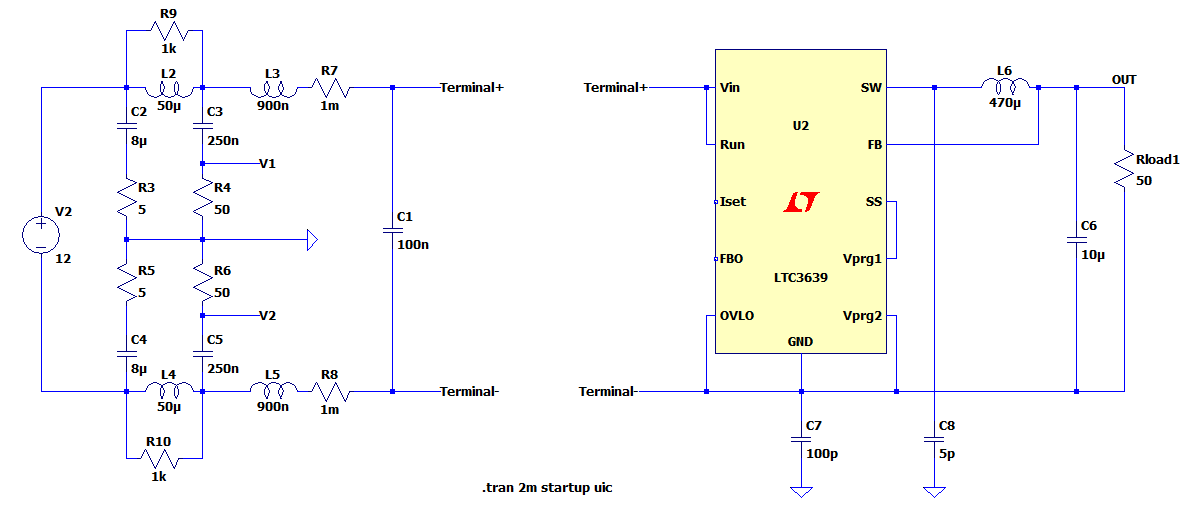
\includegraphics[width=0.8\linewidth]{Figure/LTC3639OhneFilter.png}
    \caption{LTC3639 ohne Filter}
    \label{fig:LTC3639OhneFilter}
\end{figure}

\subsection{FFT}

In Abbildung \ref{fig:LTC3639OhneFilterFFT} ist der FFT-Plot der Schaltung ohne Filter zu sehen. Hier zeigt sich, dass die Common-Mode- und Differential-Mode-Interferenzen deutlich über den zulässigen Grenzwerten für die EMV-Zertifizierung liegen. Ohne die Filterung treten hohe Störpegel auf, die die elektromagnetische Verträglichkeit der Schaltung negativ beeinflussen und eine Nicht-Zulassung für die EMV-Zertifizierung zur Folge haben würden.


\begin{figure}[H]
    \centering
    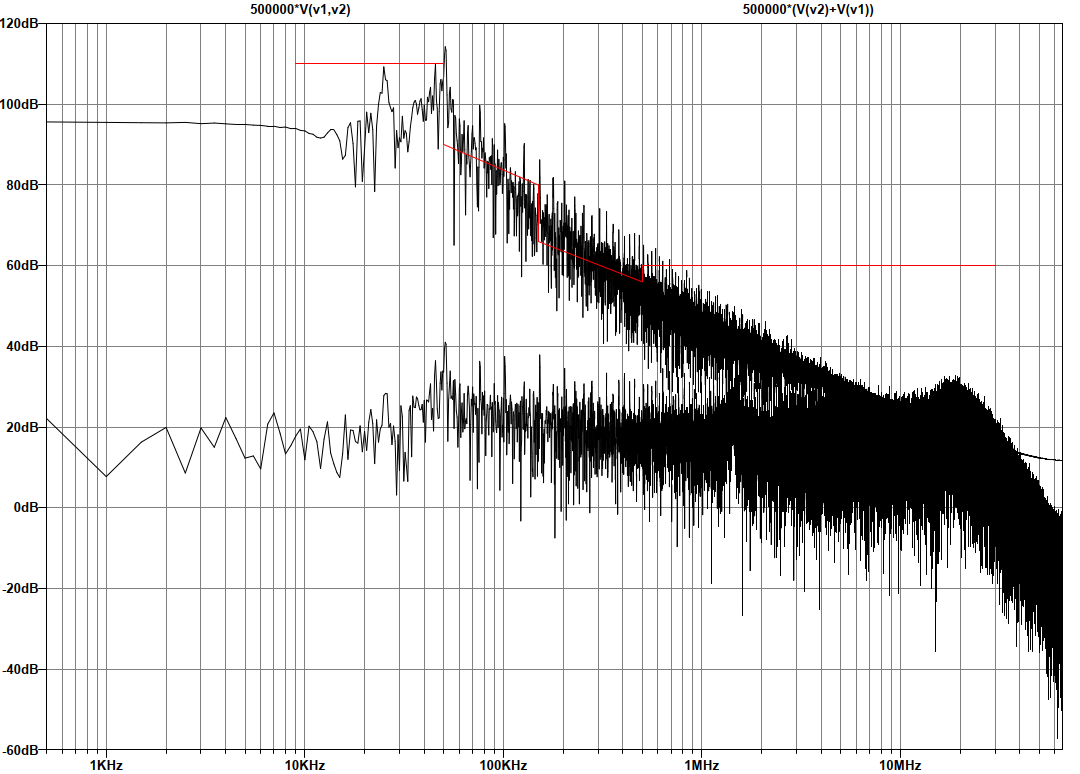
\includegraphics[width=0.8\linewidth]{Figure/LTC3639OhneFilterFFT.png}
    \caption{LTC3639 ohne Filter}
    \label{fig:LTC3639OhneFilterFFT}
\end{figure}


